% FULL REWRITE 2026-03-13 22:11 ET
\documentclass[12pt]{article}

\usepackage[margin=1in]{geometry}
\usepackage{setspace}
\usepackage[T1]{fontenc}
\usepackage[utf8]{inputenc}
\usepackage{amsmath}
\usepackage{booktabs}
\usepackage{graphicx}
\usepackage{hyperref}
\usepackage{xcolor}

\graphicspath{{output/graphs/}}
\setstretch{1.5}

\hypersetup{
  pdftitle = {Unemployment and AI Exposure},
  pdfauthor = {Leyao},
  colorlinks = true,
  linkcolor = blue,
  urlcolor = blue
}

\begin{document}

\begin{titlepage}
    \thispagestyle{empty}
    \begin{center}
        \vspace*{0.75in}
        {\LARGE\bfseries Unemployment and AI Exposure\par}
        \vspace{0.9in}
        {\Large Leyao\par}
        \vspace{0.35in}
        {\large Advisor: [Advisor Name]\par}
        \vspace{0.9in}
        {\large
            Submitted to the \\
            Distinguished Majors Program \\
            Department of Economics \\
            University of Virginia
        \par}
        \vspace{1in}
        {\large \today\par}
    \end{center}
\end{titlepage}

\newpage
\thispagestyle{empty}
\begin{center}
    {\Large\bfseries Unemployment and AI Exposure\par}
    \vspace{1.5em}
    {\large Leyao\par}
    \vspace{0.5em}
    {\normalsize \today\par}
\end{center}

\vspace{2em}
\noindent \textbf{Abstract.} This file is a working thesis scaffold for the unemployment analysis. It uses a simple thesis-style layout, includes every unemployment plot currently in the project, and separates the main table from the appendix table so the structure is ready for a longer write-up.

\par\vspace{2em}\noindent
\textbf{Keywords:} unemployment, AI exposure, labor markets
\par\noindent
\textbf{JEL Classification:} J21, J23, O33

\newpage

\section{Introduction}

This section should introduce the main question, explain why unemployment responses to AI exposure matter, and preview the contribution of the thesis. A final draft can open with the broad labor-market motivation and then narrow to the unemployment margin studied in the figures and tables below.

\section{Background}

This section can summarize the relevant background on technological change, labor-market adjustment, and the role of AI exposure in shaping worker outcomes. It is also a natural place to review related literature and describe the economic intuition behind the analysis.

\section{Data}

This section should describe the sample, the unemployment outcome, the AI exposure measure, the time period, and any controls or fixed effects used in the regressions. It can also document how the analytical sample differs across figures and tables if that matters for interpretation.

\section{Empirical Strategy}

The core unemployment specification can be summarized with a regression of the form
\begin{equation}
Unemployment_{it} = \alpha + \beta_{2024}(AIExposure_i \times 1[t=2024]) + \beta_{2025}(AIExposure_i \times 1[t=2025]) + X_{it}'\Gamma + \varepsilon_{it}.
\end{equation}

This section should explain the identifying variation, the role of controls and fixed effects, and how the appendix specification extends the main result shown in the body of the thesis.

\section{Results}

This section contains every unemployment-related plot currently available in the project and the main unemployment regression table.

\subsection{Unemployment Plots}

\begin{figure}[htbp]
    \centering
    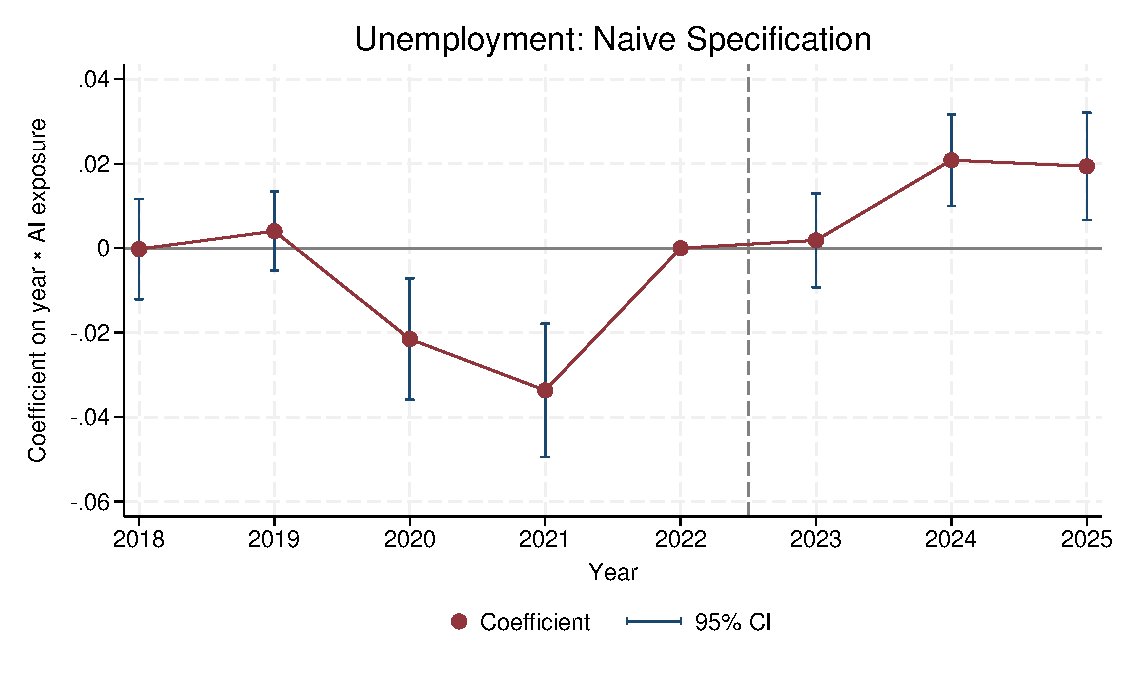
\includegraphics[width=0.9\textwidth]{unemployment_naive_plot.pdf}
    \caption{Unemployment plot, baseline specification.}
    \label{fig:unemployment_naive_plot}
\end{figure}

\begin{figure}[htbp]
    \centering
    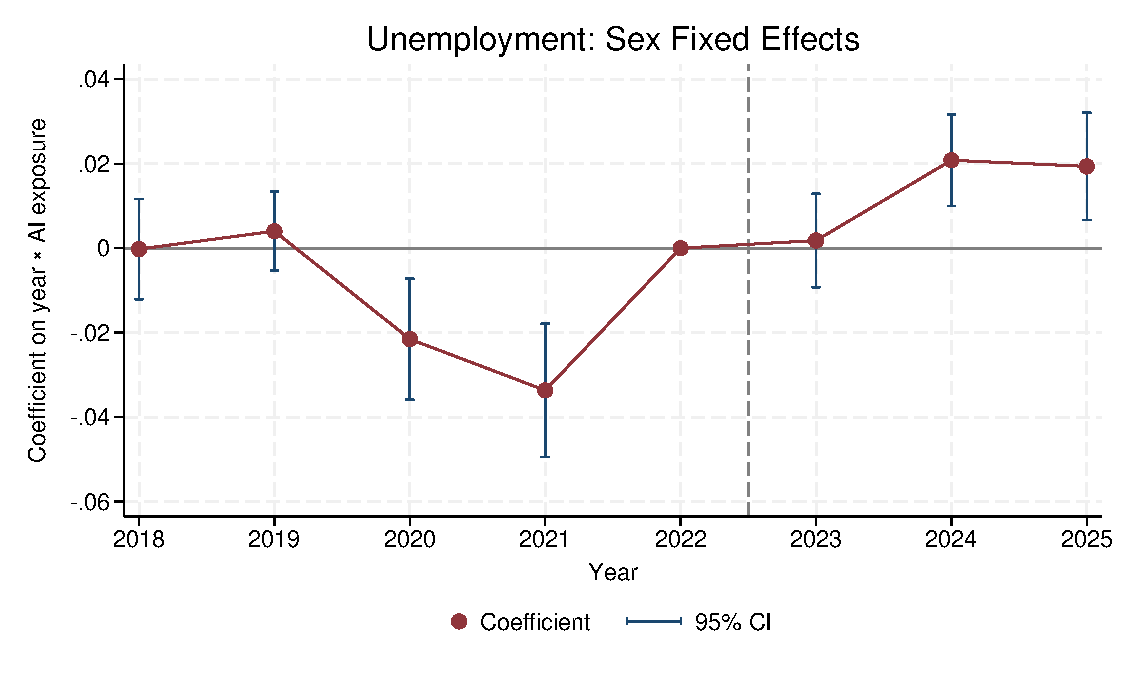
\includegraphics[width=0.9\textwidth]{unemployment_sexFE_plot.pdf}
    \caption{Unemployment plot with sex fixed effects.}
    \label{fig:unemployment_sexfe_plot}
\end{figure}

\begin{figure}[htbp]
    \centering
    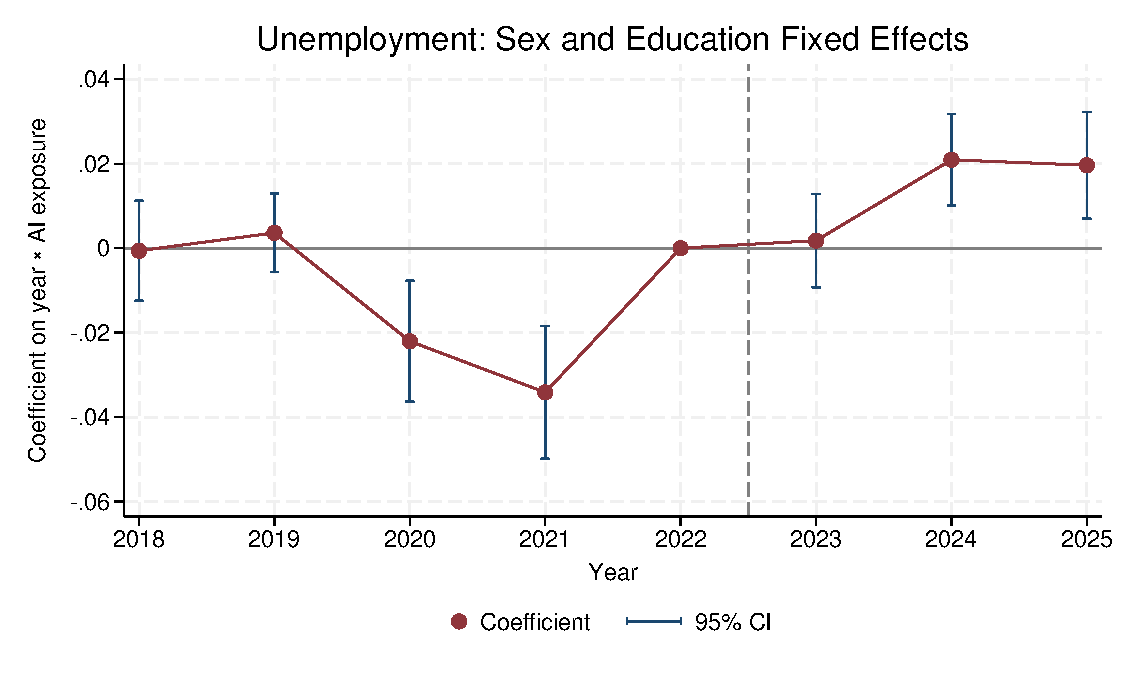
\includegraphics[width=0.9\textwidth]{unemployment_sexeducFE_plot.pdf}
    \caption{Unemployment plot with sex and education fixed effects.}
    \label{fig:unemployment_sexeducfe_plot}
\end{figure}

\begin{figure}[htbp]
    \centering
    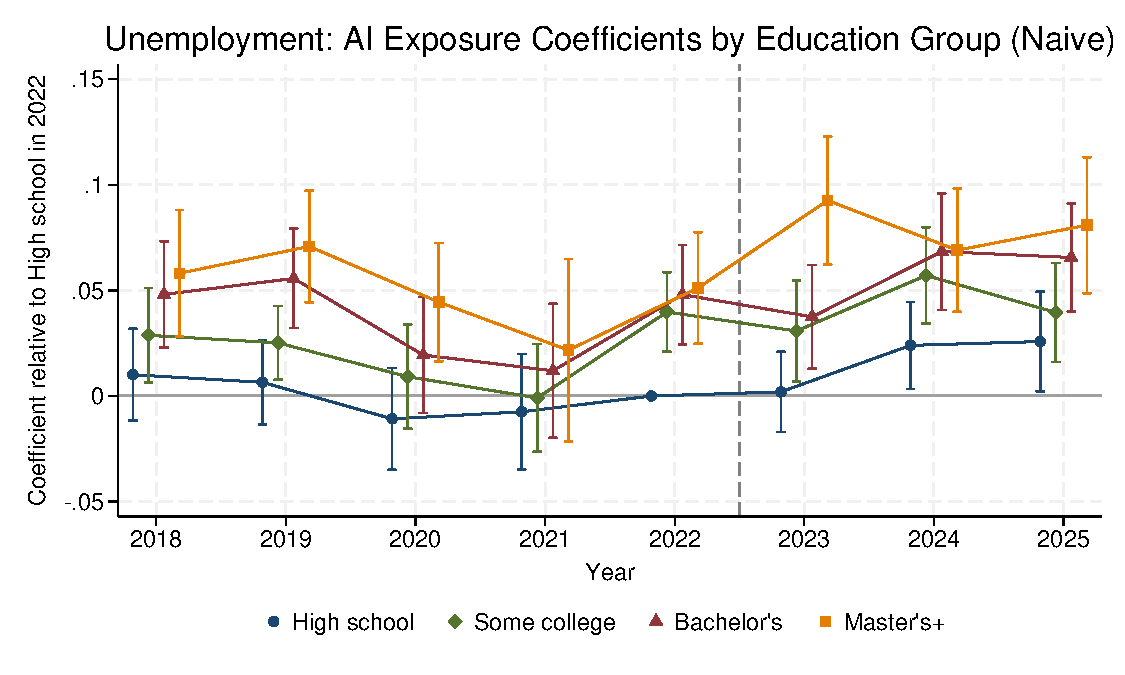
\includegraphics[width=0.9\textwidth]{unemployment_ai_educ_naive.pdf}
    \caption{Unemployment and AI exposure by education, baseline specification.}
    \label{fig:unemployment_ai_educ_naive}
\end{figure}

\begin{figure}[htbp]
    \centering
    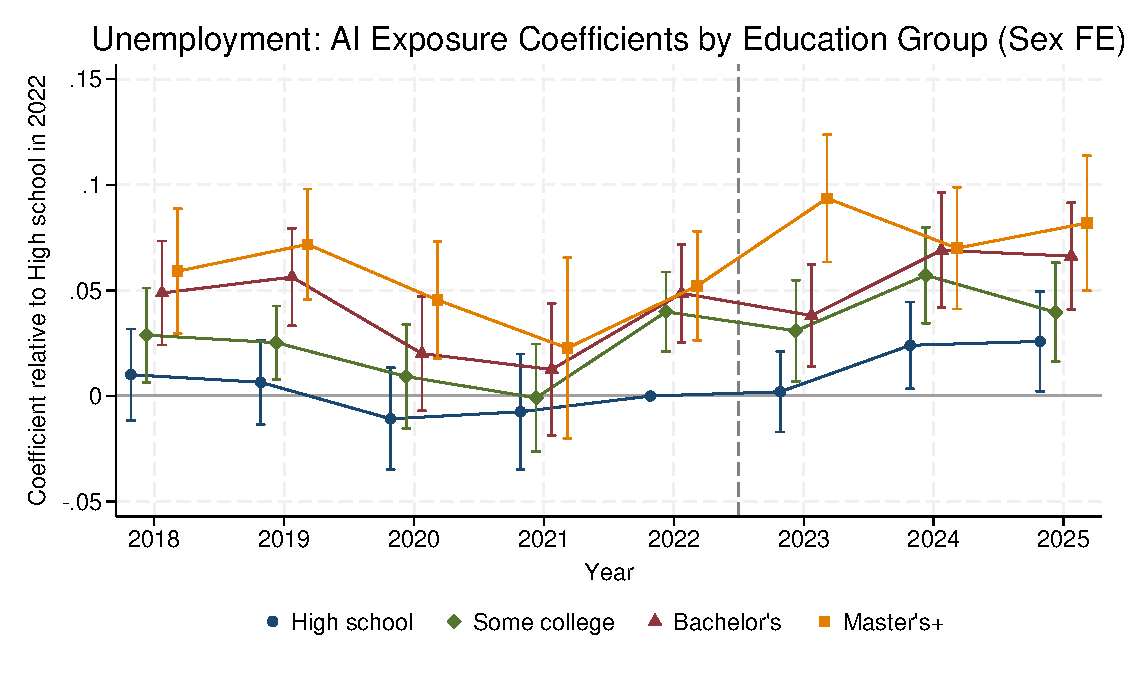
\includegraphics[width=0.9\textwidth]{unemployment_ai_educ_sexFE.pdf}
    \caption{Unemployment and AI exposure by education with sex fixed effects.}
    \label{fig:unemployment_ai_educ_sexfe}
\end{figure}

\begin{figure}[htbp]
    \centering
    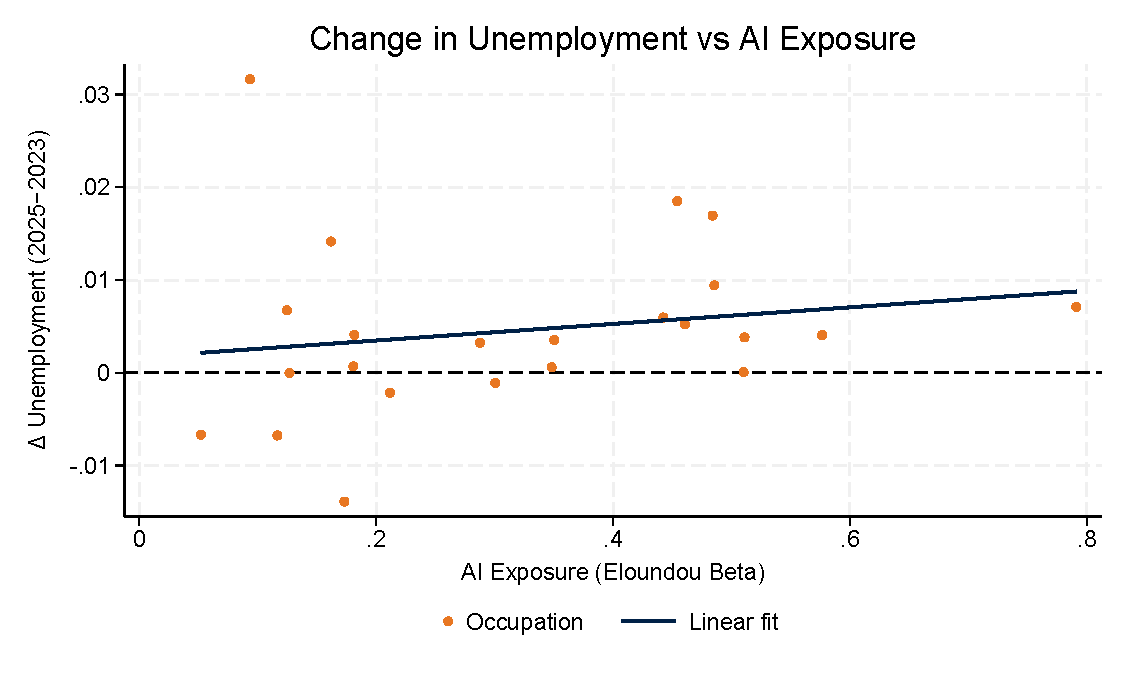
\includegraphics[width=0.9\textwidth]{delta_unemp_2023-2025.pdf}
    \caption{Change in unemployment from 2023 to 2025.}
    \label{fig:delta_unemployment_2023_2025}
\end{figure}

\subsection{Main Table}

\begin{table}[htbp]
    \centering
    \caption{Main unemployment regression results}
    \label{tab:unemployment_main}
    \resizebox{0.9\textwidth}{!}{\def\sym#1{\ifmmode^{#1}\else\(^{#1}\)\fi}
\begin{tabular}{l*{4}{c}}
\toprule
Dependent Variable: & \multicolumn{4}{c}{Unemployment} \\
\cmidrule(lr){2-5}
 & (1) & (2) & (3) & (4) \\
\midrule
2018 $\times$ AI exposure&   -0.000228   &   -0.000216   &   -0.000606   &  -0.0000988   \\
            &   (0.00603)   &   (0.00604)   &   (0.00602)   &   (0.00607)   \\
2019 $\times$ AI exposure&     0.00404   &     0.00403   &     0.00362   &     0.00364   \\
            &   (0.00478)   &   (0.00477)   &   (0.00473)   &   (0.00471)   \\
2020 $\times$ AI exposure&     -0.0215***&     -0.0215***&     -0.0220***&     -0.0215***\\
            &   (0.00729)   &   (0.00729)   &   (0.00728)   &   (0.00720)   \\
2021 $\times$ AI exposure&     -0.0337***&     -0.0337***&     -0.0341***&     -0.0355***\\
            &   (0.00802)   &   (0.00802)   &   (0.00801)   &   (0.00801)   \\
2023 $\times$ AI exposure&     0.00184   &     0.00182   &     0.00179   &     0.00155   \\
            &   (0.00566)   &   (0.00564)   &   (0.00563)   &   (0.00554)   \\
2024 $\times$ AI exposure&      0.0208***&      0.0208***&      0.0209***&      0.0208***\\
            &   (0.00554)   &   (0.00553)   &   (0.00553)   &   (0.00554)   \\
2025 $\times$ AI exposure&      0.0194***&      0.0194***&      0.0196***&      0.0180***\\
            &   (0.00647)   &   (0.00647)   &   (0.00643)   &   (0.00633)   \\
\midrule
Mean of dependent variable&       0.034   &       0.034   &       0.034   &       0.034   \\
Sex FE      &          No   &         Yes   &         Yes   &         Yes   \\
Education FE&          No   &          No   &         Yes   &         Yes   \\
State $\times$ Year FE&          No   &          No   &          No   &         Yes   \\
SE clustered at&  Occupation   &  Occupation   &  Occupation   &  Occupation   \\
Observations&     500,669   &     500,669   &     500,669   &     500,669   \\
\bottomrule
\end{tabular}
}
\end{table}

\clearpage
\section{Interpretation}

This section can discuss the economic magnitude of the unemployment effects, compare the visual evidence in the plots to the regression evidence in the table, and explain whether the results are robust across specifications with richer controls.

\section{Conclusion}

This section can summarize the main takeaway, explain how the unemployment analysis fits into the broader thesis argument, and note the most important limitations or next steps.

\clearpage
\appendix
\section{Appendix}

This section is reserved for supplementary material and keeps the appendix unemployment table separate from the main table in the results section.

\subsection{Appendix Table}

\begin{table}[htbp]
    \centering
    \caption{Appendix unemployment regression results}
    \label{tab:unemployment_appendix}
    \resizebox{0.9\textwidth}{!}{\def\sym#1{\ifmmode^{#1}\else\(^{#1}\)\fi}
\begin{tabular}{l*{4}{c}}
\toprule
Dependent Variable: & \multicolumn{4}{c}{Unemployment} \\
\cmidrule(lr){2-5}
 & (1) & (2) & (3) & (4) \\
\midrule
2018 $\times$ Experience $\times$ AI exposure&    0.000415   &    0.000415   &    0.000408   &    0.000413   \\
            &  (0.000368)   &  (0.000368)   &  (0.000370)   &  (0.000369)   \\
2019 $\times$ Experience $\times$ AI exposure&    0.000905***&    0.000905***&    0.000887** &    0.000895***\\
            &  (0.000349)   &  (0.000349)   &  (0.000345)   &  (0.000342)   \\
2020 $\times$ Experience $\times$ AI exposure&    0.000546   &    0.000545   &    0.000535   &    0.000526   \\
            &  (0.000348)   &  (0.000348)   &  (0.000343)   &  (0.000341)   \\
2021 $\times$ Experience $\times$ AI exposure&    0.000697*  &    0.000696*  &    0.000705*  &    0.000722** \\
            &  (0.000358)   &  (0.000358)   &  (0.000359)   &  (0.000354)   \\
2023 $\times$ Experience $\times$ AI exposure&    0.000457   &    0.000456   &    0.000442   &    0.000430   \\
            &  (0.000377)   &  (0.000377)   &  (0.000378)   &  (0.000378)   \\
2024 $\times$ Experience $\times$ AI exposure&  0.00000951   &  0.00000826   &   0.0000324   &   0.0000509   \\
            &  (0.000386)   &  (0.000387)   &  (0.000387)   &  (0.000387)   \\
2025 $\times$ Experience $\times$ AI exposure&    0.000336   &    0.000335   &    0.000341   &    0.000337   \\
            &  (0.000410)   &  (0.000410)   &  (0.000409)   &  (0.000408)   \\
\midrule
Mean of dependent variable&       0.034   &       0.034   &       0.034   &       0.034   \\
Sex FE      &          No   &         Yes   &         Yes   &         Yes   \\
Education FE&          No   &          No   &         Yes   &         Yes   \\
State $\times$ Year FE&          No   &          No   &          No   &         Yes   \\
SE clustered at&  Occupation   &  Occupation   &  Occupation   &  Occupation   \\
Observations&     500,669   &     500,669   &     500,669   &     500,669   \\
\bottomrule
\end{tabular}
}
\end{table}

\end{document}
